\section{global.c File Reference}
\label{global_8c}\index{global.c@{global.c}}
{\tt \#include $<$stdio.h$>$}\par
{\tt \#include \char`\"{}filter.h\char`\"{}}\par
{\tt \#include \char`\"{}conversion.h\char`\"{}}\par
{\tt \#include \char`\"{}ueac.h\char`\"{}}\par
{\tt \#include \char`\"{}external\_\-flash.h\char`\"{}}\par
{\tt \#include \char`\"{}ueaclib.h\char`\"{}}\par
{\tt \#include \char`\"{}timer.h\char`\"{}}\par


Include dependency graph for global.c:\begin{figure}[H]
\begin{center}
\leavevmode
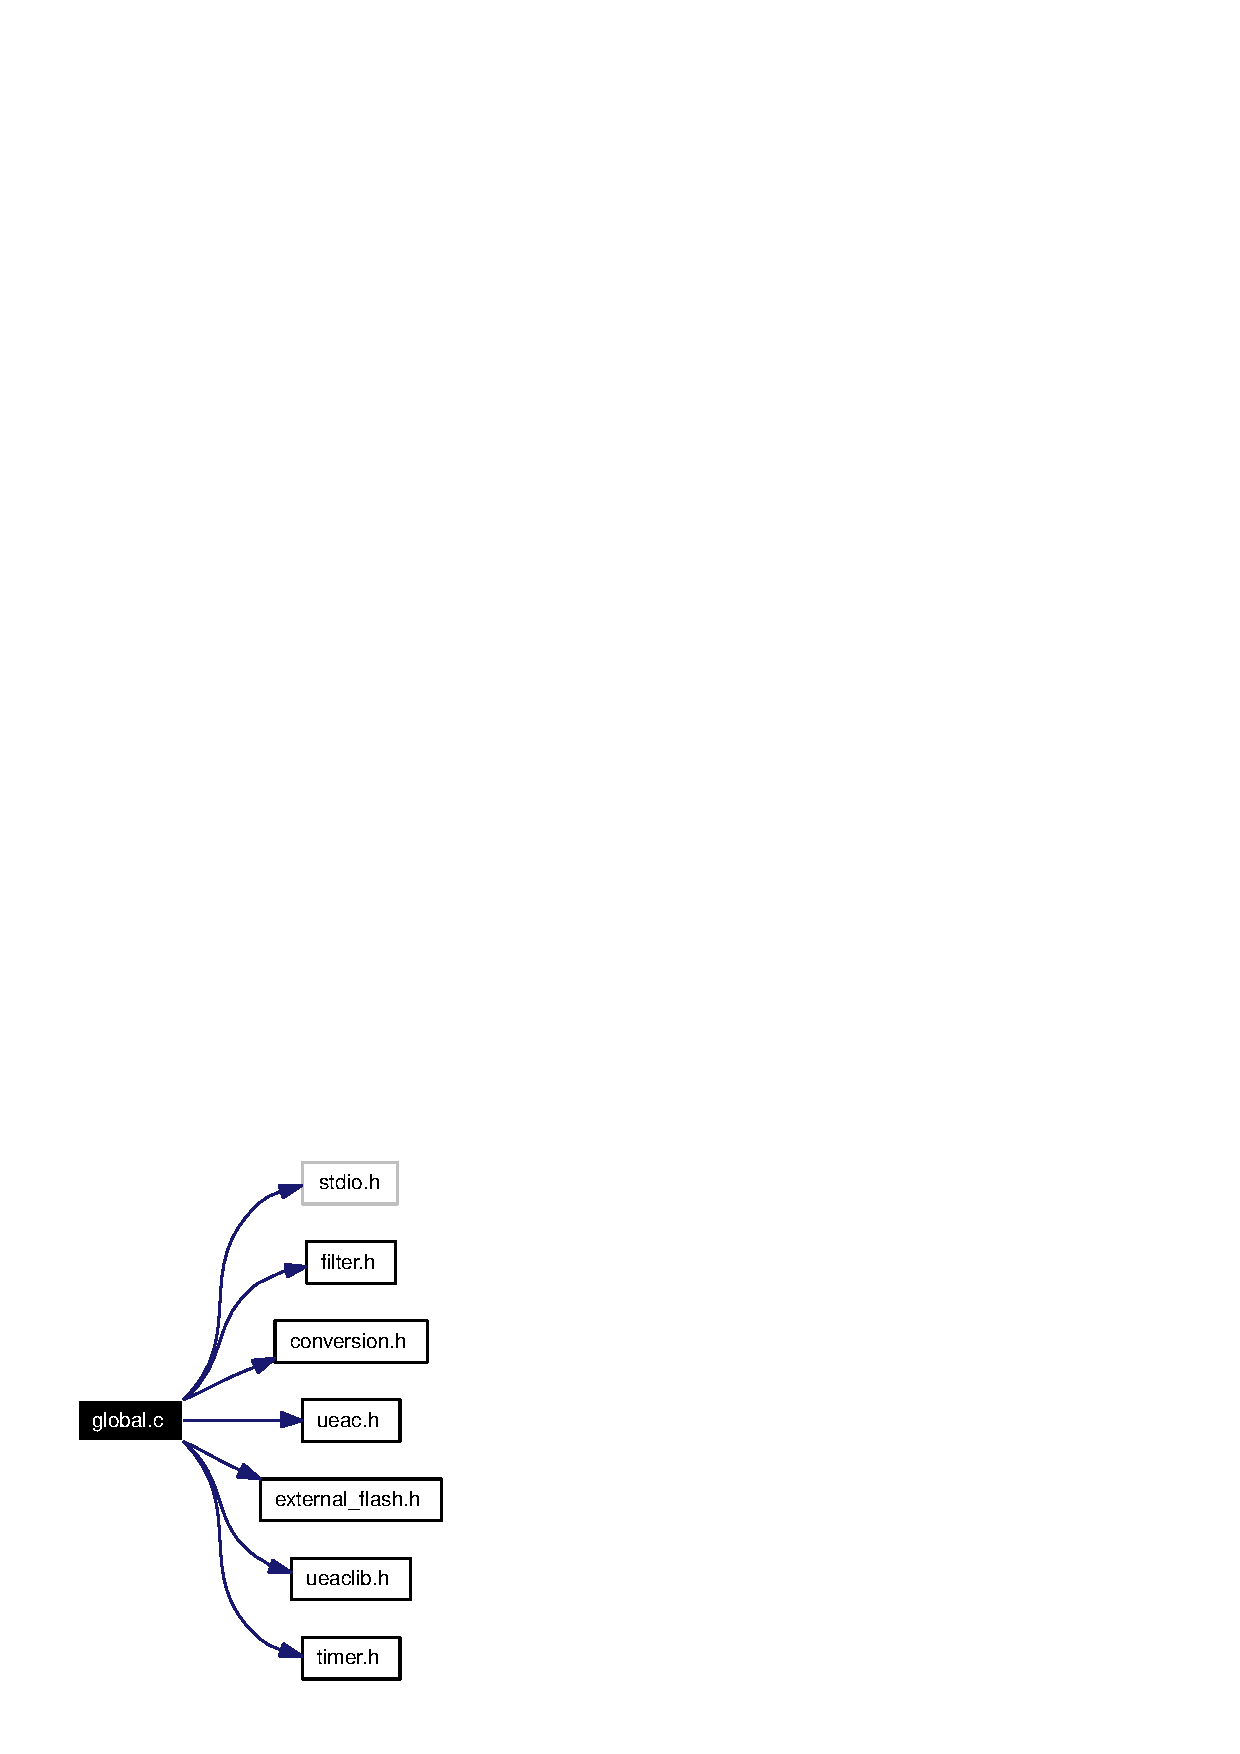
\includegraphics[width=106pt]{global_8c__incl}
\end{center}
\end{figure}
\subsection*{Defines}
\begin{CompactItemize}
\item 
\#define {\bf LLA\_\-TABLE}~{\bf ueac\_\-state} $\rightarrow$ lla\_\-table
\end{CompactItemize}
\subsection*{Functions}
\begin{CompactItemize}
\item 
void {\bf init\_\-pin\_\-data\_\-structure} (void)
\item 
void {\bf init\_\-ueac\_\-state\_\-structure} (void)
\item 
void {\bf init\_\-global\_\-variables} (void)
\end{CompactItemize}
\subsection*{Variables}
\begin{CompactItemize}
\item 
{\bf ueac\_\-t} {\bf ueac\_\-state}
\item 
char {\bf command} [100]
\item 
{\bf channel\_\-t} {\bf pin\_\-data} [25]
\item 
{\bf ueacval\_\-t} {\bf conversion\_\-result}
\item 
volatile int {\bf timer\_\-tick}
\item 
unsigned char {\bf led\_\-screen\_\-enable} = 0
\item 
unsigned char {\bf high\_\-time\_\-limit} [25]
\end{CompactItemize}


\subsection{Define Documentation}
\index{global.c@{global.c}!LLA_TABLE@{LLA\_\-TABLE}}
\index{LLA_TABLE@{LLA\_\-TABLE}!global.c@{global.c}}
\subsubsection{\setlength{\rightskip}{0pt plus 5cm}\#define LLA\_\-TABLE~{\bf ueac\_\-state} $\rightarrow$ lla\_\-table}\label{global_8c_a0}




Definition at line 66 of file global.c.

Referenced by evaluate\_\-lla(), lla\_\-add(), lla\_\-disable(), lla\_\-enable(), lla\_\-print\_\-active(), and lla\_\-report().

\subsection{Function Documentation}
\index{global.c@{global.c}!init_global_variables@{init\_\-global\_\-variables}}
\index{init_global_variables@{init\_\-global\_\-variables}!global.c@{global.c}}
\subsubsection{\setlength{\rightskip}{0pt plus 5cm}void init\_\-global\_\-variables (void)}\label{global_8c_a10}




Definition at line 121 of file global.c.

References init\_\-pin\_\-data\_\-structure(), init\_\-ueac\_\-state\_\-structure(), led\_\-screen\_\-enable, and timer\_\-tick.

Referenced by main().

\footnotesize\begin{verbatim}121                                   {
122   init_pin_data_structure();   
123   init_ueac_state_structure();
124   timer_tick=0;
125   led_screen_enable=0;
126 }
\end{verbatim}\normalsize 




Here is the call graph for this function:\begin{figure}[H]
\begin{center}
\leavevmode
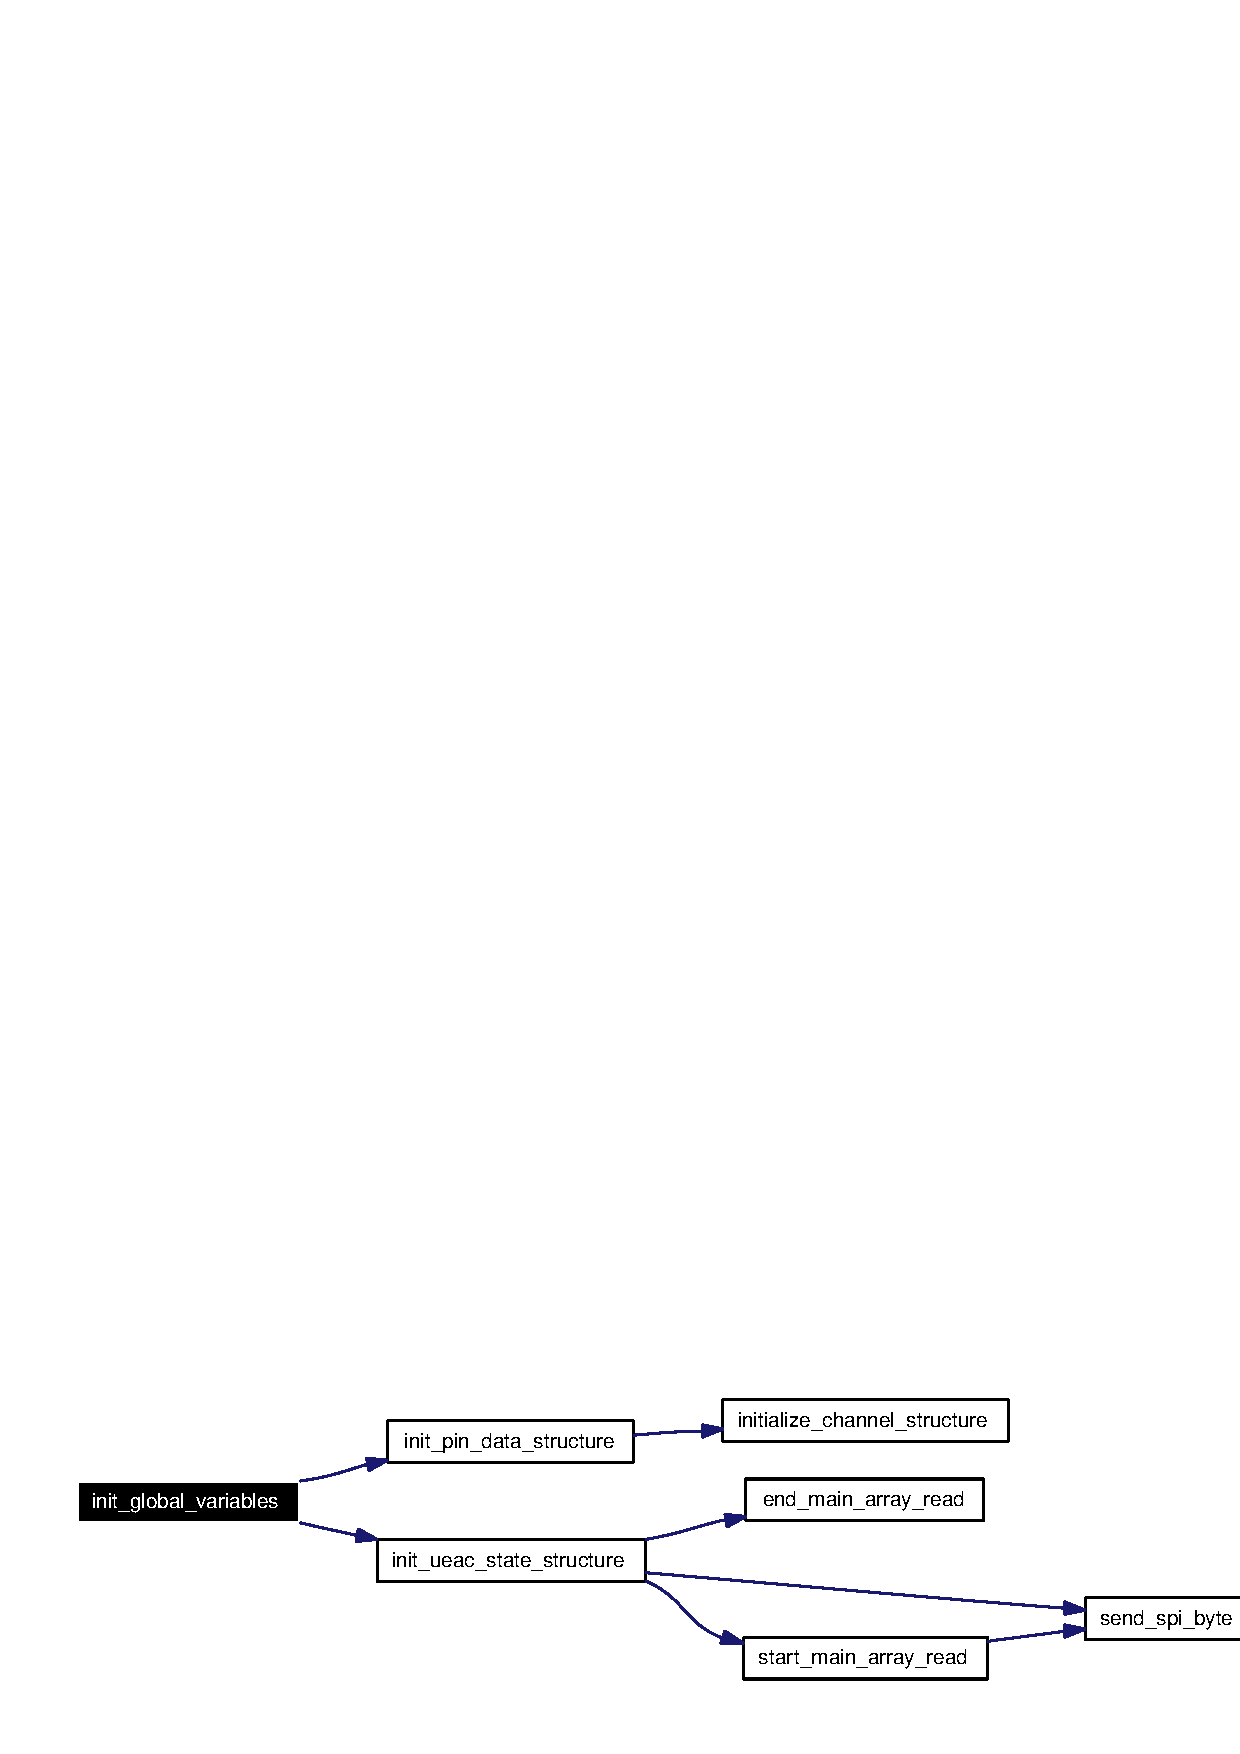
\includegraphics[width=301pt]{global_8c_a10_cgraph}
\end{center}
\end{figure}
\index{global.c@{global.c}!init_pin_data_structure@{init\_\-pin\_\-data\_\-structure}}
\index{init_pin_data_structure@{init\_\-pin\_\-data\_\-structure}!global.c@{global.c}}
\subsubsection{\setlength{\rightskip}{0pt plus 5cm}void init\_\-pin\_\-data\_\-structure (void)}\label{global_8c_a8}




Definition at line 68 of file global.c.

References initialize\_\-channel\_\-structure().

Referenced by init\_\-global\_\-variables().

\footnotesize\begin{verbatim}68                                    {
69   int i;
70   for (i=0;i<25;i++) {
71     initialize_channel_structure(&pin_data[i]);
72   }
73 }
\end{verbatim}\normalsize 




Here is the call graph for this function:\begin{figure}[H]
\begin{center}
\leavevmode
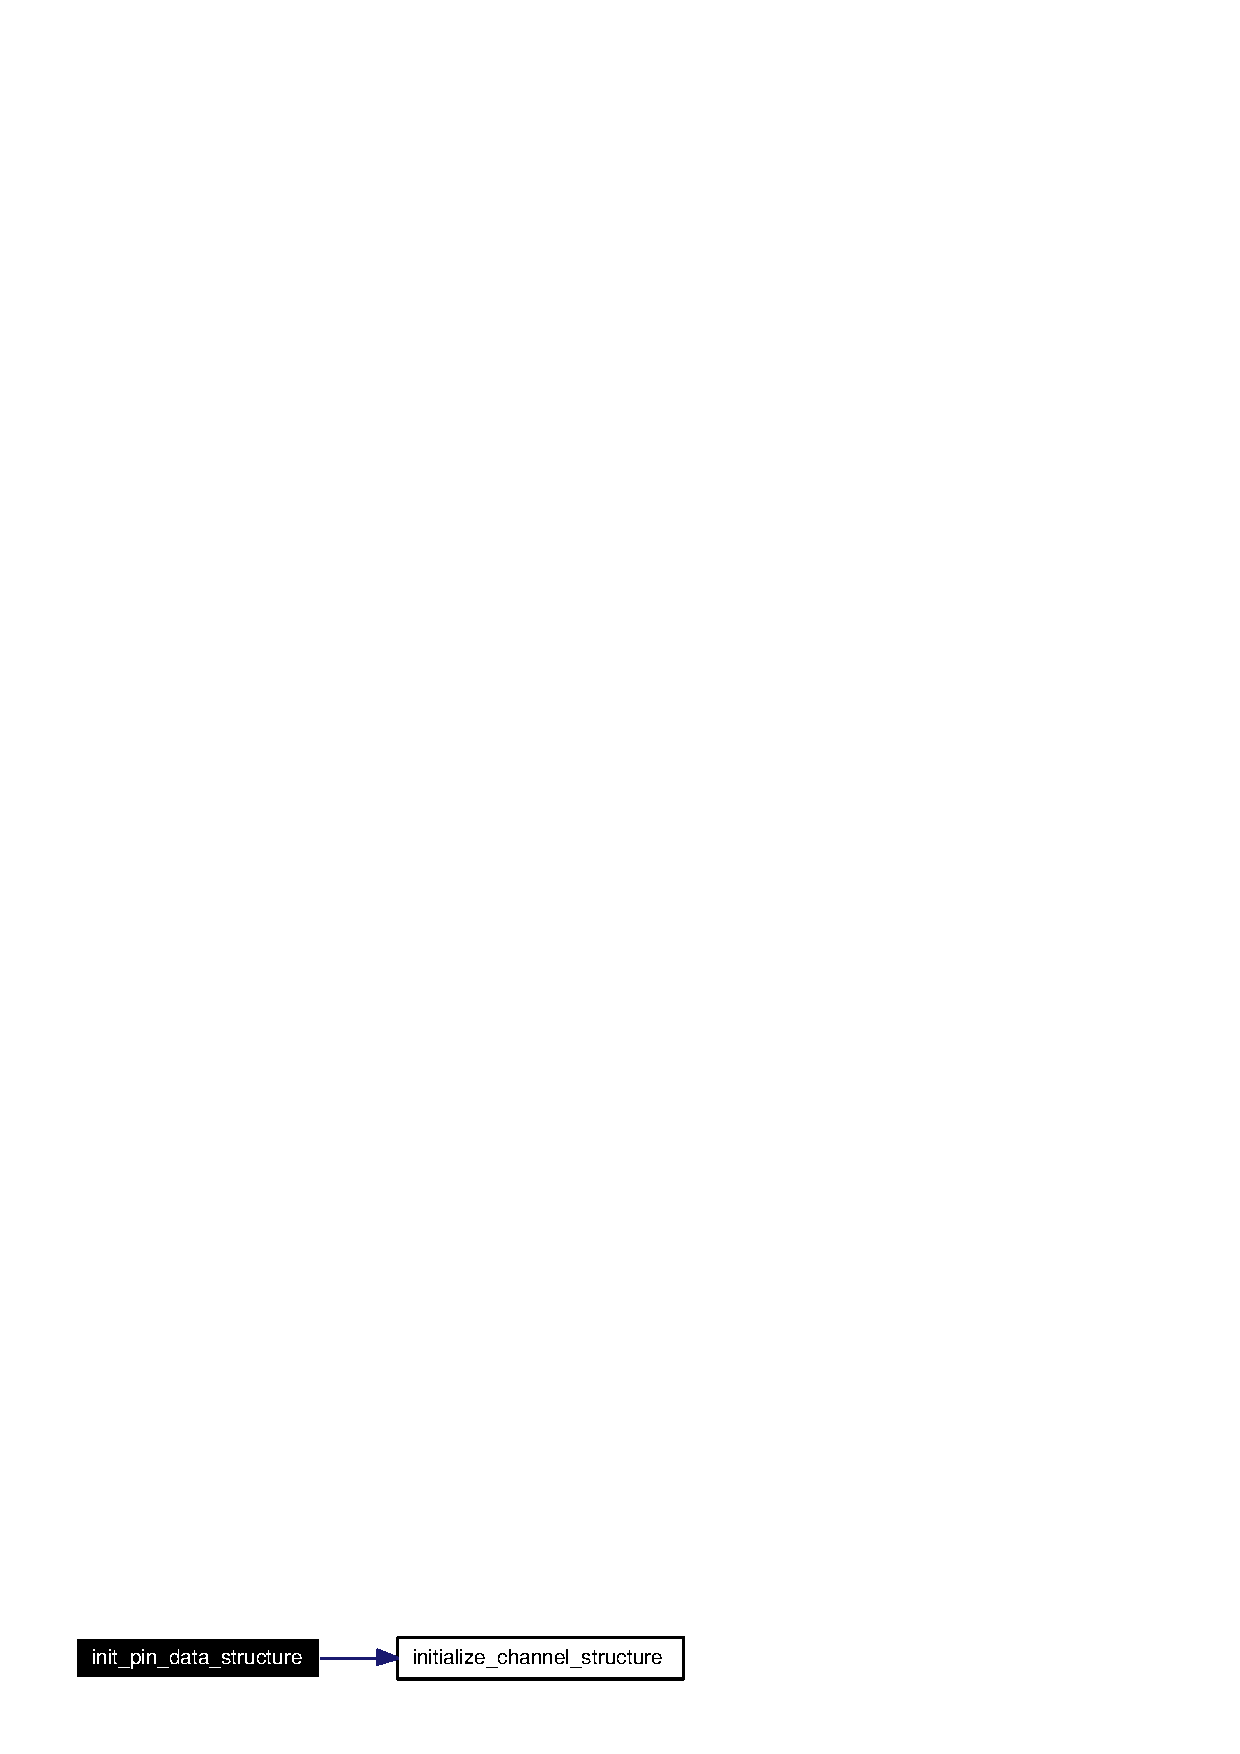
\includegraphics[width=164pt]{global_8c_a8_cgraph}
\end{center}
\end{figure}
\index{global.c@{global.c}!init_ueac_state_structure@{init\_\-ueac\_\-state\_\-structure}}
\index{init_ueac_state_structure@{init\_\-ueac\_\-state\_\-structure}!global.c@{global.c}}
\subsubsection{\setlength{\rightskip}{0pt plus 5cm}void init\_\-ueac\_\-state\_\-structure (void)}\label{global_8c_a9}




Definition at line 75 of file global.c.

References end\_\-main\_\-array\_\-read(), cal::i\_\-200u\-A\_\-offset, cal::i\_\-in\_\-floor, cal::i\_\-in\_\-offset, cal::i\_\-zero\_\-offset, lla::in\_\-pin, ueac::lla\_\-input, ueac::lla\_\-table, lla::out\_\-pin, ueac::pin\_\-cal, ueac::pin\_\-current, send\_\-spi\_\-byte(), and start\_\-main\_\-array\_\-read().

Referenced by init\_\-global\_\-variables().

\footnotesize\begin{verbatim}75                                      {
76   int i;
77   char ch; 
78   ueac_state.lla_input=0;
79   for (i=0;i<25;i++) {
80     ueac_state.pin_current[i]=0;
81     ueac_state.lla_table[i].in_pin=0xFF;
82     ueac_state.lla_table[i].out_pin=0xFF;
83   }
84 
85   // Load calibration data from external flash
86   start_main_array_read(0,0); 
87   ch=send_spi_byte(0);
88   if (ch=='V') {
89     // valid calibration, proceed with load
90     for (i=0;i<25;i++) {
91       ueac_state.pin_cal[i].i_200uA_offset=(char)send_spi_byte(0);
92     }
93     for (i=0;i<25;i++) {
94       ueac_state.pin_cal[i].i_zero_offset=(char)send_spi_byte(0);
95     }
96     for (i=0;i<25;i++) {
97       ueac_state.pin_cal[i].i_in_floor=(char)send_spi_byte(0);
98     }
99     for (i=0;i<25;i++) {
100       ueac_state.pin_cal[i].i_in_offset=(char)send_spi_byte(0);
101     }
102     end_main_array_read();
103     //    for (i=0;i<25;i++) {
104     //  printf ("%d %d ",i,ueac_state.pin_cal[i].i_200uA_offset);
105     //  printf ("%d ",ueac_state.pin_cal[i].i_zero_offset);
106     //  printf ("%d ",ueac_state.pin_cal[i].i_in_floor);
107     //  printf ("%d\n\r",ueac_state.pin_cal[i].i_in_offset);
108     //    }     
109   }
110   else {
111     // no cal, load defaults 
112     for (i=0;i<25;i++) {
113       ueac_state.pin_cal[i].i_200uA_offset=0x00;
114       ueac_state.pin_cal[i].i_zero_offset=0x00;
115       ueac_state.pin_cal[i].i_in_floor=0x00;
116       ueac_state.pin_cal[i].i_in_offset=0x00;
117     }
118   }
119 }
\end{verbatim}\normalsize 




Here is the call graph for this function:\begin{figure}[H]
\begin{center}
\leavevmode
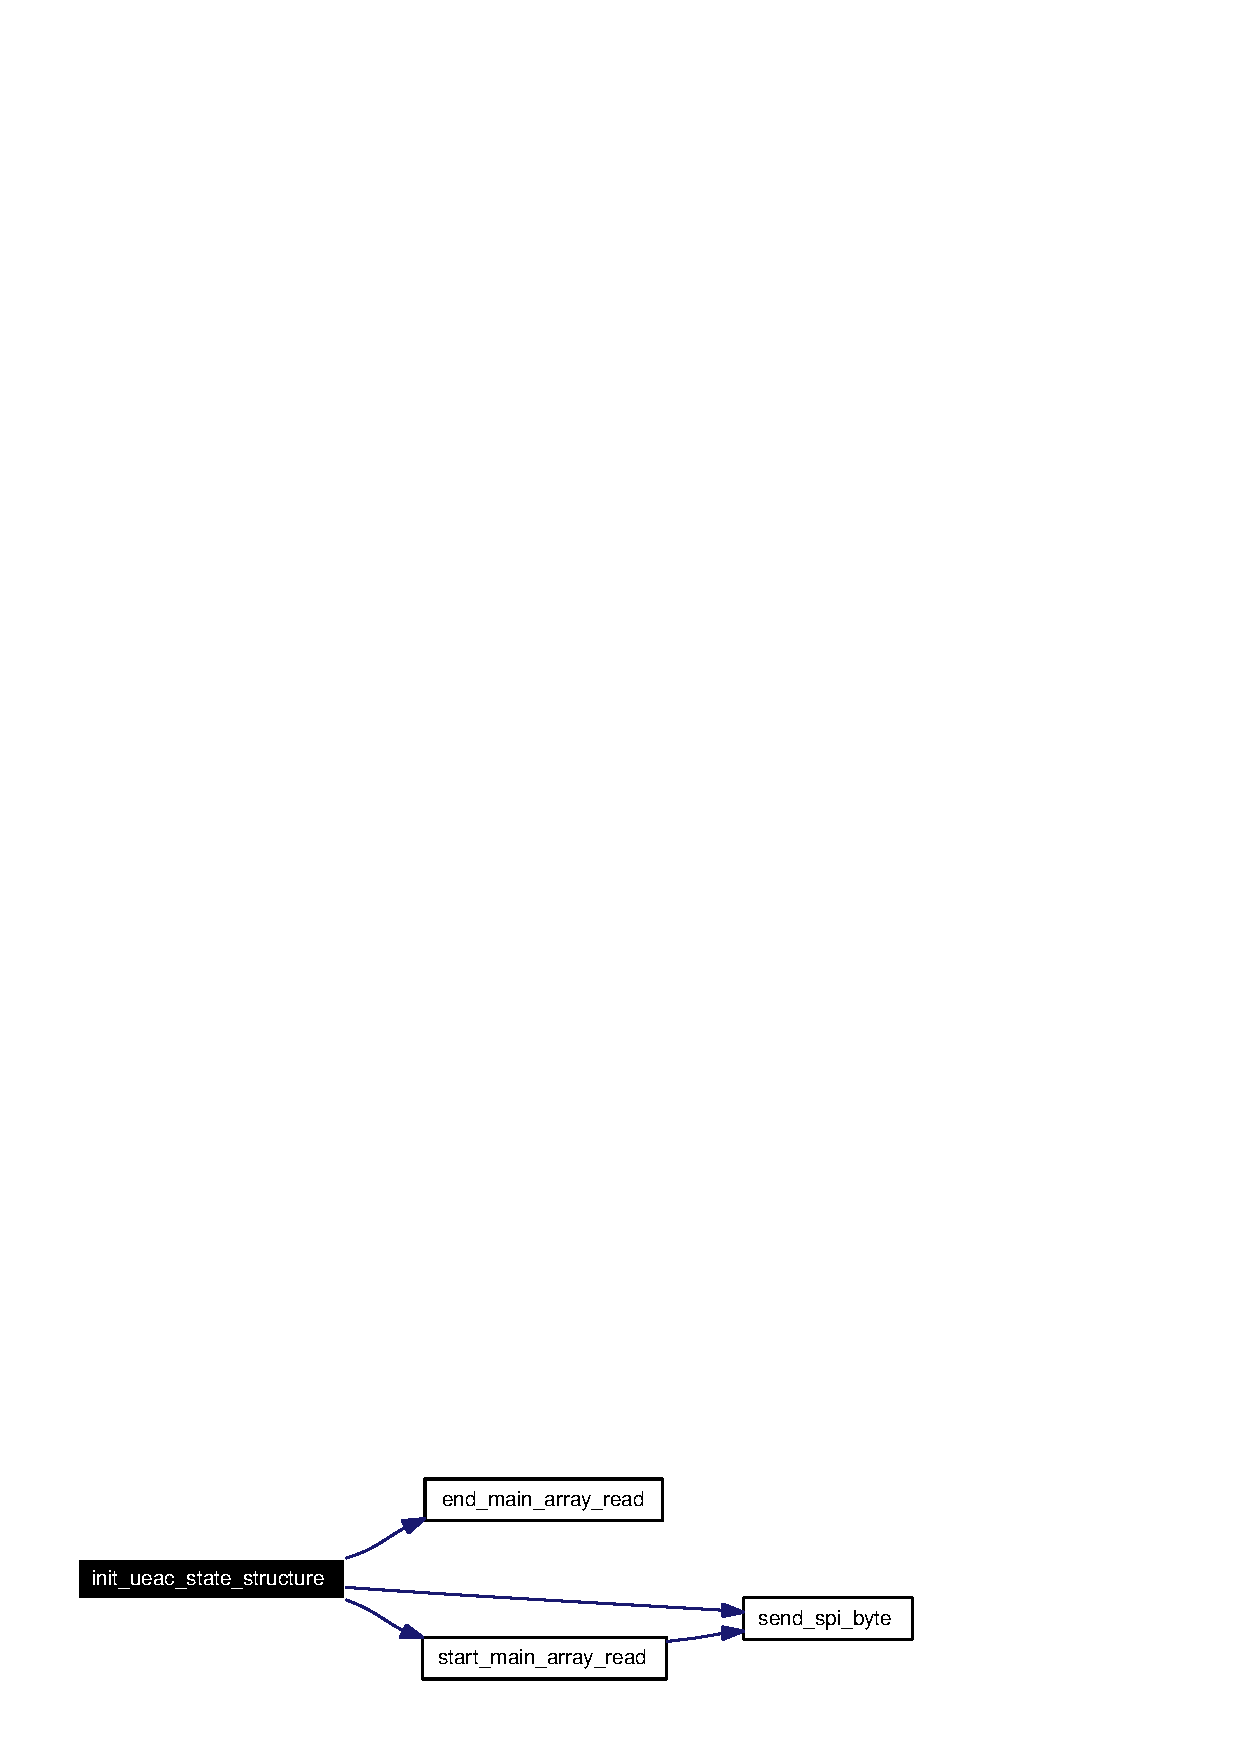
\includegraphics[width=219pt]{global_8c_a9_cgraph}
\end{center}
\end{figure}


\subsection{Variable Documentation}
\index{global.c@{global.c}!command@{command}}
\index{command@{command}!global.c@{global.c}}
\subsubsection{\setlength{\rightskip}{0pt plus 5cm}char {\bf command}[100]}\label{global_8c_a2}




Definition at line 55 of file global.c.

Referenced by main().\index{global.c@{global.c}!conversion_result@{conversion\_\-result}}
\index{conversion_result@{conversion\_\-result}!global.c@{global.c}}
\subsubsection{\setlength{\rightskip}{0pt plus 5cm}{\bf ueacval\_\-t} {\bf conversion\_\-result}}\label{global_8c_a4}




Definition at line 57 of file global.c.

Referenced by print\_\-grid\_\-i(), print\_\-grid\_\-v(), scan\_\-probes(), and ueac\_\-execute\_\-instruction().\index{global.c@{global.c}!high_time_limit@{high\_\-time\_\-limit}}
\index{high_time_limit@{high\_\-time\_\-limit}!global.c@{global.c}}
\subsubsection{\setlength{\rightskip}{0pt plus 5cm}unsigned char {\bf high\_\-time\_\-limit}[25]}\label{global_8c_a7}


{\bf Initial value:}

\footnotesize\begin{verbatim} {1,1,1,1,1,
                                     1,1,1,1,1,
                                     1,1,1,1,1,
                                     1,1,1,1,1,
                                     1,1,1,1,2}
\end{verbatim}\normalsize 


Definition at line 60 of file global.c.

Referenced by led\_\-pwm(), and timer\_\-a0\_\-irq().\index{global.c@{global.c}!led_screen_enable@{led\_\-screen\_\-enable}}
\index{led_screen_enable@{led\_\-screen\_\-enable}!global.c@{global.c}}
\subsubsection{\setlength{\rightskip}{0pt plus 5cm}unsigned char {\bf led\_\-screen\_\-enable} = 0}\label{global_8c_a6}




Definition at line 59 of file global.c.

Referenced by init\_\-global\_\-variables(), main(), timer\_\-a0\_\-irq(), and ueac\_\-execute\_\-instruction().\index{global.c@{global.c}!pin_data@{pin\_\-data}}
\index{pin_data@{pin\_\-data}!global.c@{global.c}}
\subsubsection{\setlength{\rightskip}{0pt plus 5cm}{\bf channel\_\-t} {\bf pin\_\-data}[25]}\label{global_8c_a3}




Definition at line 56 of file global.c.

Referenced by current\_\-output\_\-calibration(), evaluate\_\-lla(), print\_\-grid\_\-i(), print\_\-grid\_\-v(), scan\_\-probes(), timer\_\-a0\_\-irq(), and ueac\_\-execute\_\-instruction().\index{global.c@{global.c}!timer_tick@{timer\_\-tick}}
\index{timer_tick@{timer\_\-tick}!global.c@{global.c}}
\subsubsection{\setlength{\rightskip}{0pt plus 5cm}volatile int {\bf timer\_\-tick}}\label{global_8c_a5}




Definition at line 58 of file global.c.

Referenced by delay\_\-1\_\-25m\-S(), init\_\-global\_\-variables(), and timer\_\-a0\_\-irq().\index{global.c@{global.c}!ueac_state@{ueac\_\-state}}
\index{ueac_state@{ueac\_\-state}!global.c@{global.c}}
\subsubsection{\setlength{\rightskip}{0pt plus 5cm}{\bf ueac\_\-t} {\bf ueac\_\-state}}\label{global_8c_a1}




Definition at line 54 of file global.c.

Referenced by convert\_\-a2d(), main(), timer\_\-a0\_\-irq(), ueac\_\-execute\_\-instruction(), and write\_\-current().